\documentclass[a4paper,10pt, jcp, aps, preprint]{revtex4-1}

\usepackage[utf8]{inputenc}
\usepackage{amsmath, amsfonts}
\usepackage{graphicx}
\usepackage{natbib}
\usepackage{caption}
\usepackage{subcaption}
\usepackage{authblk}

\bibliographystyle{alpha}

%opening
\title{Exact kinetics of two hard discs in a rectangular box}
\author{Rosa Rodríguez \& David P.~Sanders \& W. P. K. Zapfe}
\affil{Departamento de Física, Facultad de Ciencias, Universidad Nacional Autónoma de México, Ciudad Universitaria, Del.~Coyoacán, México D.F. 04510, Mexico}

\usepackage{mathptmx}

\newcommand{\defeq}{:=}
\newcommand{\mean}[1]{\left \langle #1 \right \rangle}
\newcommand{\rd}{\, \mathrm{d}}
\newcommand{\RR}{\mathbb{R}}
\newcommand{\vv}{\mathbf{v}}
\newcommand{\indicator}[1]{\mathbf{1}_{ \{   #1 \} } } 

\setlength{\parskip}{10pt}
\setlength{\parindent}{0pt}

\begin{document}

\maketitle

\begin{abstract}
  We obtain exact results for the kinetics of the inertial motion of 
two hard discs in a rectangular two-dimensional box.
  In particular,  we calculate exactly the mean hopping time between exchanges
 of the horizontal positions of the discs, 
as well as mean collision rates between the two discs and 
 between the discs and the box. We compare this with numerical experiments.
\end{abstract}

\section{Introduction}

Hard sphere billiards are one of the most recurred models in
statistical physics and non linear dynamics.  Some of the simplest models
 provide us with a deep mathematical understanding
about the qualitative aspects of their evolution, such as 
the properties under the moniker \emph{Hard Chaos} (
hyperbolicity, ergodicity and mixing qualities). One such system is the
gas of disks in a rectangular box, a two dimensional realisation of a
hard sphere gas. It is known that such a system is chaotic in the
strong sense \cite{Sinai70}. 
For the statistical physicist, \emph{mean} and \emph{first} encounter
times are of uttermost importance, as many properties,
such as mixing rates and the physical origin of a positive
Liapunov exponent, depend on it. 


The minimal realisation of this
system consists in two disks of same mass and radius inside a 
rectangular box. This system displays hard chaos and 
is amenable to treatment using
results from ergodic theory \cite{Sinai70, Gallavotti74, SzaszBook00}. 


\section{Model}

We consider two discs of radius $r$ (and diameter $d=2r$) 
in a box of width $w$ and height $h$ (figure
\ref{billar01}). 
The discs move inertially in the absence of forces, 
following straight line trajectories,
and undergo elastic collisions with each 
other and with the walls of the box.

\begin{figure}[h]
  \centering
  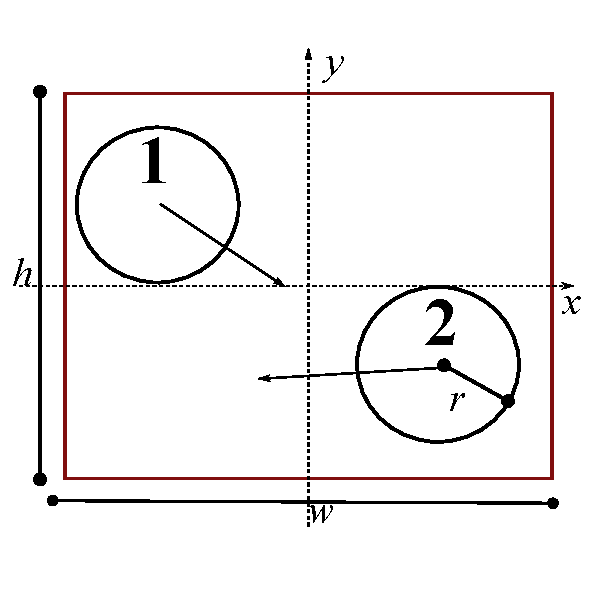
\includegraphics[width=0.56\textwidth]{DiscosenCajaCuadrada01.pdf}
  \caption{The Billiard}\label{billar01}
\end{figure}


We denote the position of the centre of the $i$th disc by 
$(x_{i}, y_{i})$ for $i=1,2$. Since the discs are hard, 
the disc centres are restricted to the region 
$(x_i, y_i) \in [-a,a] \times [-b, b]$, where 
$a \defeq a(d) \defeq \frac{w}{2} - r = \frac{w-d}{2}$ and
 $b \defeq b(d) \defeq \frac{h}{2} - r = \frac{h-d}{2}$.


The exclusion condition is $(x_1-x_2)^2 + (y_1-y_2)^2 \ge (2r)^2 = d^2$.
It is thus useful to work in terms of the new coordinates
\begin{equation}\label{cambiocoor01}
 x \defeq \frac{x_1 - x_2}{\sqrt{2}}; 
\quad X \defeq \frac{x_1 + x_2}{\sqrt{2}}; 
\quad y \defeq \frac{y_1 - y_2}{\sqrt{2}}; 
\quad Y \defeq \frac{y_1 + y_2}{\sqrt{2}}.
\end{equation}


In these coordinates the conditions are rewritten as
$x \in [-a \sqrt{2}, +a \sqrt{2}]$ with 
$X \in [-a \sqrt{2} + |x|, a \sqrt{2} - |x|]$, respectively 
 $y \in [-b \sqrt{2}, b \sqrt{2}]$ and $Y \in [-b \sqrt{2} + |y|, +b \sqrt{2} - |y|]$,  
with the constraint $x^2 + y^2 \ge \frac{d^2}{2}$.

The exclusions define a hypercube with a hypercylinder inside, placed diagonally 
from one hyperarista to its opposite. 
The dynamics in such a space follow
the usual billiard rules: free flight until
encounter with a wall, then elastic reflection.
The outer borders are flat, so the
hyperbolicity is due only to the inner dispersing
boundary \cite{Sim99}, which represents the coalition of
two disks in the original space.


\subsection{Assumptions for the Collision Rates}

This kind of systems are equivalent to Bernoulli Flows \cite{Gallavotti74}.
For such systems is expected an exponential decay of 
distributions \cite{AbadiGalves} with potentially
long algebraic tails \cite{ZasTip}. 
This includes recurrence times and
first encounter times. 

There are two apparently similar but frustratingly different events.
If we want to calculate a \emph{Recurrence time} for the collisions 
between the two disks, 
we should depart from the subset of all outgoing trajectories from the surface of the
hyper-cylinder. 
If we want to calculate the \emph{first} encounter time, then
this supposition is not necessary.
 Actually, this complicates
the model, as there are no general results or 
techniques to describe this collision in continuous time. 


 

\section{Mean time between events}

A system of $N$ hard spheres confined by hard walls in a $d$ dimensional
space may be treated as a billiard system 
in which a single point  particle undergoes free motion between reflecting obstacles 
in a $ d N $-dimensional configuration space \cite{Sinai70, MarkChern}. 

If the resulting billiard is ergodic and hyperbolic, then we
have a result for the mean free time, i.e.\ the mean time between 
collisions of the particle with the walls \cite{MarkChern}. 
This can be thought of as a mean return time to the $(d-1)$-dimensional 
(i.e. co-dimension-$1$) cross-section given by the wall boundaries.
The formula for this is
\begin{equation}\label{meanfreetime}
 \mean{\tau} = \frac{|Q|}{|A|} \frac{|S^{d-1}|}{|B^{d-1}|}.
\end{equation}
Here $|Q|$ denotes the $d$-dimensional volume of the available 
space in the billiard and 
$|A|$ the $(d-1)$-dimensional area of the cross-section.
 $|S^{d-1}|$ is the $(d-1)$-dimensional area of the unit sphere in $\RR^d$ given by
\begin{equation}
  |S^{d-1}| = \frac{2 \pi^{d/2}}{\Gamma(d/2)},
\end{equation}
where $\Gamma(\cdot)$ is the gamma function. 
$|B^{d-1}|$ is the volume of the unit ball 
in $\RR^{d-1}$, given by $|B^{d-1}| = |S^{d-2}| / (d-1)$.
In the formula \ref{meanfreetime}  the particle has 
its velocity scaled to unity.

Machta and Zwanzig \cite{MachtaZwan} used a similar method to derive an escape 
time across a non-existent boundary by treating it as a recurrence time.
Since it is an escape time, they used velocities whose components point only 
perpendicularly to the ``exit wall''.

In our case, we are interested in the mean return time to 
a co-dimension-$1$ cross section, 
which is defined by the exact moment
in which the disk interchange their horizontal position. This is simply
\begin{equation} \label{condchoque}
x_1 = x_2.
\end{equation}

Given that each disk has different momentum, but
they can interchange it without affecting the
total energy, we must take into account the mass $m$ of each disk 
and the total kinetic energy $E$.
If both discs have the same mass then $\sum_i \vv_i^2 = 2E / m$.
The above result, as derived by Chernov, 
was for the case $\sum_i \vv_i^2 = 1$, or $m=1$ and $E=\frac{1}{2}$.  
For more general values of $E$ and $m$, 
we are simply working on a different energy surface in phase space. 
The particle trajectories are identical but their motion is a factor
$\sqrt{2E/m}$ faster, so that all times are divided by this value, 
giving for
the mean time between events the general formula:
\begin{equation} \label{meantimegeneral}
  \mean{\tau} =  \frac{1}{\sqrt{2E / m}} 
\frac{|Q| \, |S^3|} {|A| \, |B^3|}.	
\end{equation}
In our particular case, the efective dimension is four,
and $E=m=1$, so that the general factor of the formula appear as:
\begin{equation} \label{meantimegeneral}
   \frac{1}{\sqrt{2E / m}} 
\frac{|S^3|}{|B^3|}=\frac{3\pi}{2\sqrt{2}}.	 
\end{equation}

The next step is obtaining the Volume (4 dimensional measure) of
the available space and the Area (3 dimensional induced measure) of
the collision conditions. We devote the next section to
detail the procedure.


\section{Calculation of Volumes and Areas}

The configuration
space is an hypercube with an hyper-cylinder subtracted in a diagonal position.
The uncomfortable part is to deal with the tips of the cylinder, which
present the  shape of a wedge with a circular base and two 
orthogonal ``heights''. 
The calculation can be carried out indirectly, using indicator functions for the
available space or for the  prohibited space.

\subsection{Volume of available space}

We shall present the total four-dimensional volume as a product integral
of all available positions. To better grasp the idea, a convenient
diagram is shown in the next figure, (\ref{diagintegra01}).

\begin{figure}[h]
  \centering
  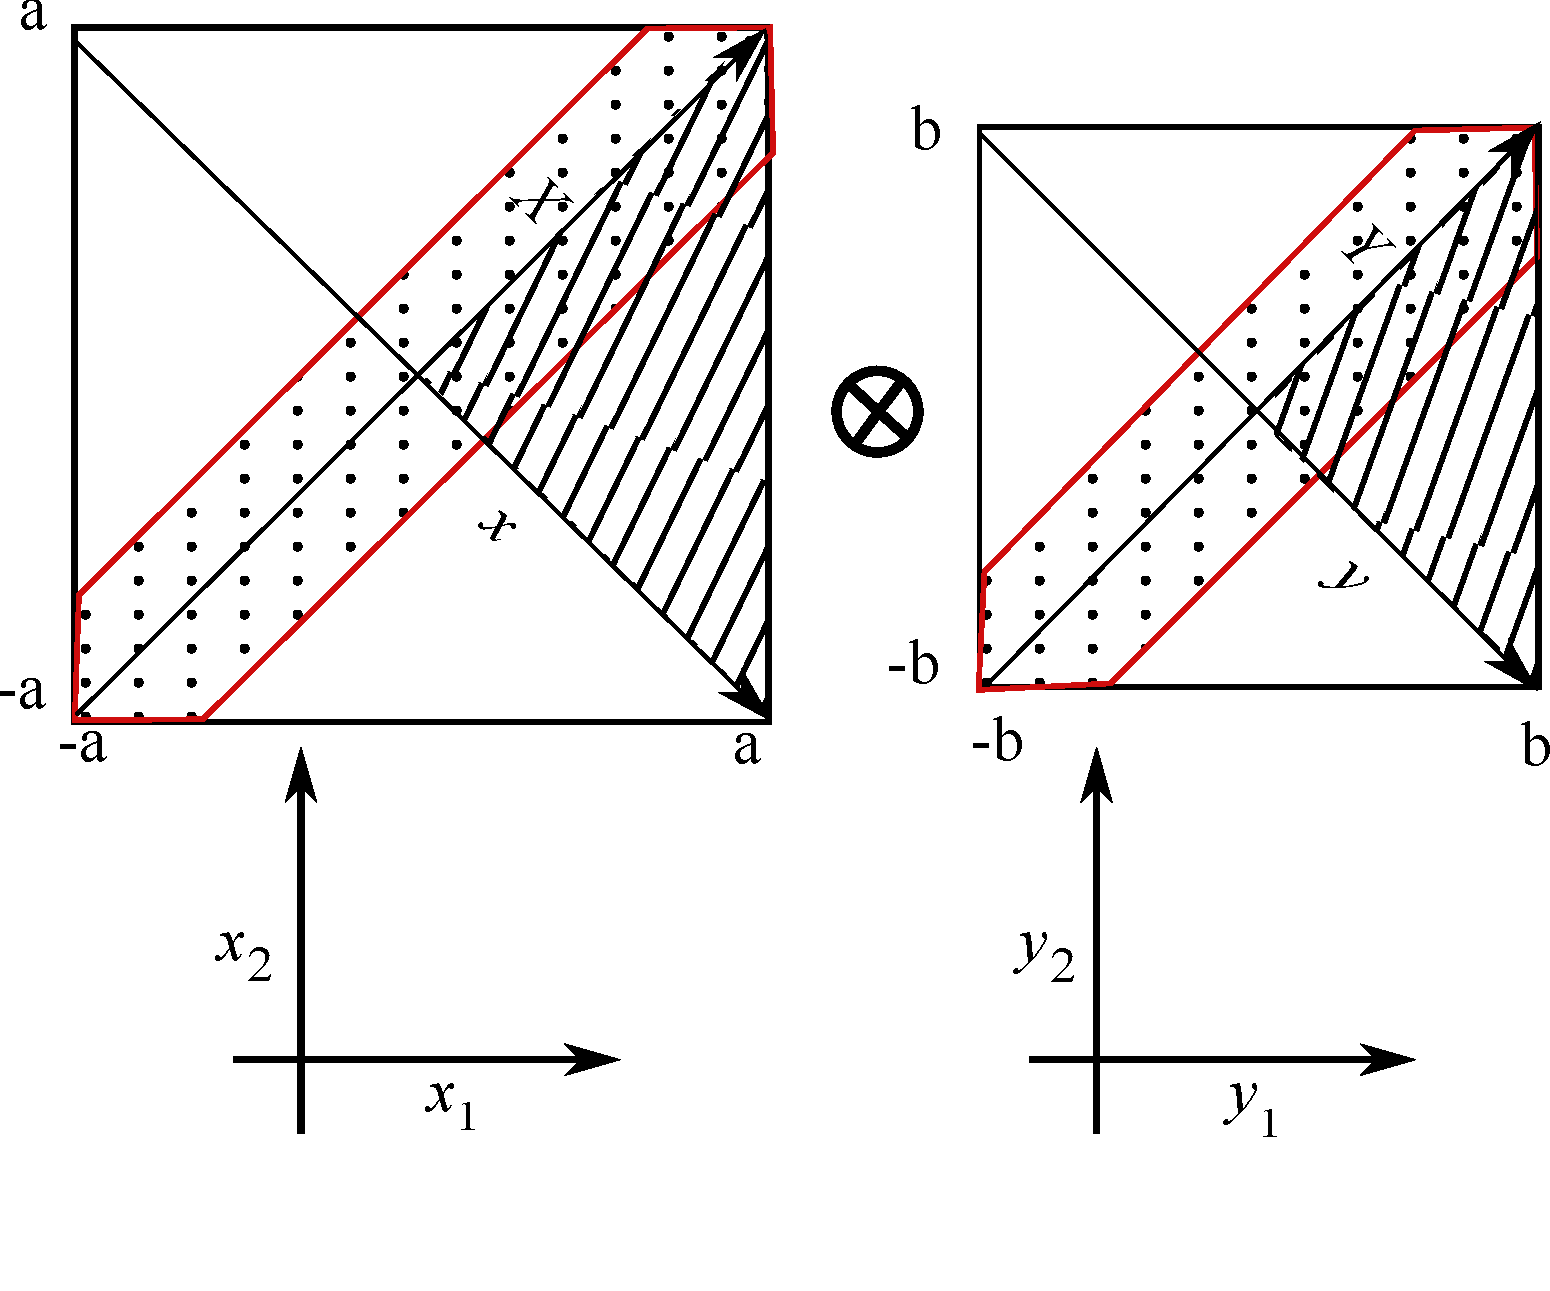
\includegraphics[width=0.75\textwidth]{diagramintegra01.pdf}
  \caption{The space to integrate is the product of the subspaces
    belonging to horizontal and vertical coordinates. The colour
    shaded area represents the ``exclusion'' set, where the condition 
    $ (x_1-x_2)^2 + (y_1-y_2)^2 \ge d^2 $ is not fulfilled. 
    Their width is dependent on the particular point of evaluation
    on the \emph{other} subspace. The diagonal coordinates
    make the expression to evaluate simpler. Due to 
    symmetry, we only evaluate the area in stripes and
    multiply the result by 16.}\label{diagintegra01}
\end{figure}

\begin{equation}\label{volindic}
 V = \int_{x_1 = -a}^a \rd x_1 \int_{x_2 = -a}^a \rd x_2 
\int_{y_1 = -b}^b \rd y_1 \int_{y_2 = -b}^b \rd y_2 \, \indicator{ (x_1-x_2)^2 + (y_1-y_2)^2 \ge d^2 },
\end{equation}
where $\indicator{Z}$ indicates the indicator function of the set $Z$, given by $\mathbf{1}_Z (x) = 1$ if $x \in Z$, and $=0$ if $x \notin Z$, which restricts the integral to the desired region $Z$.

We represent the excluded cylinder in the coordinates defined in 
the set of equation \ref{cambiocoor01}. 

\begin{equation}\label{integraltotal}
 V = \int_{x=-a \sqrt{2}}^{a \sqrt{2}} \rd x 
\int_{X=-a \sqrt{2} + |x| }^{a \sqrt{2} - |x|}  \rd X
 \int_{y=-b \sqrt{2}}^{b \sqrt{2}} \rd y
\int_{Y=-b \sqrt{2} + |y| }^{b \sqrt{2}-|y|}  \rd Y
\, \indicator{ x^2 + y^2 \ge \frac{d^2}{2}  }.
\end{equation}
In these coordinates, $X$ and $Y$ do not appear in the integrating part, so that these integrals may be done trivially, thus reducing to the following two-dimensional integral:
\begin{align}
 V &= \int_{x=-a \sqrt{2}}^{a \sqrt{2}} \rd x  \int_{y=-b \sqrt{2}}^{b \sqrt{2}} \rd y
\, 2 \left( a \sqrt{2} - |x| \right) \, 2 \left( b \sqrt{2} - |y| \right) \,  \indicator{ x^2 + y^2 \ge \frac{d^2}{2} } \\
&= 16 \int_{x=0}^{a \sqrt{2}} \rd x  \int_{y=0}^{b \sqrt{2}} \rd y
\, \left( a \sqrt{2} - x \right) \, \left( b \sqrt{2} - y \right) \,  \indicator{ x^2 + y^2 \ge \frac{d^2}{2} },
\end{align}
using the symmetry.

Thus $V = 16(I_1 + I_2)$, where $I_1$ and $I_2$ are the resulting integrals over the regions where the available region for $y$ is affected by, and is not affected by, respectively, the restriction to lie outside the disc.
We have
\begin{align}
 I_1 &= \int_{x=0}^{d / \sqrt{2}} \left[ \int_{y = \sqrt{\frac{1}{2} {d^2} - x^2}}^{b \sqrt{2}} \left( b \sqrt{2} - y \right) \rd y \right]  \left( a \sqrt{2} - x \right) \rd x \\
&= 	
a b^{2} d + \textstyle \frac{1}{6} (a+b) d^{3} - \frac{1}{32}  d^{4} - \frac{1}{4} {\left(\pi a b + b^{2}\right)} d^{2},
\end{align}
and
\begin{align}
 I_2 &= \int_{x=d / \sqrt{2}}^{a \sqrt{2}} \left[ \int_{y = 0}^{b \sqrt{2}} \left( b \sqrt{2} - y \right) \rd y \right]  \left( a \sqrt{2} - x \right) \rd x \\
&=	
{\left( a^{2} - a d + \textstyle \frac{1}{4}  d^{2}\right)} b^{2}.
\end{align}
Thus 
\begin{equation}\label{volumeabd}
 V %= 16(I_1 + I_2) =     	
= 16 a^{2} b^{2}  - 4 \pi a b d^{2} + \textstyle \frac{8}{3} (a+b) d^{3}  - \frac{1}{2} d^{4},
\end{equation}
as was previously obtained by Munakata and Hu \cite{Munakata02}.

Note that the volume available to place two discs inside 
the hard box but \emph{without} the 
 hard-disc exclusion constraint is simply 
given by the first term, $16 a^2 b^2$; 
thus, the remaining terms represent the excluded volume due to this constraint.
The available space gets smaller nevertheless, as can be seen from
the substitutions $a\rightarrow (w-d)/2$ and $b\rightarrow (h-d)/2$.
The explicit formula for the Volume as function from the diameter only is then:

\begin{equation}\label{volumewhd}
 V 
= (w-d)^{2} (h-d)^{2}  - 
 \pi (w-d)(h-d) d^{2} + 
\textstyle \frac{4}{3} (w+h-2d) d^{3}  
- \frac{1}{2} d^{4},
\end{equation}
 
For the numeric values $w=h=1$, the biggest possible diameter is 
$d=\sqrt{2}/(1+\sqrt{2})$. Unhappily, there is a quirk in the above formula:
it stops being valid before that. The reason is that the deduction
of the formula doesn't include the case in which hopping is not possible. 
We tacitly made the assumption that $h,w>2d$.  This assumption is on 
the integration limits in the step in eq. \ref{integraltotal}. 
A full discussion of the formula for the case in which either
$w$ or $h$ are smaller than $2d$ but there is still space for
the disks is discussed elsewhere \cite{notascalculokarel}. 
We cite the  result for $h/2  <d< w/2$ for illustrative purposes.
For cleanliness we define another auxiliary variable,
$c=\sqrt{d^2-b^2}$:
\begin{multline}\label{VolumenCasoFeo}
V_{h/2<d} = 8abd^2[\arccos(b/d)-\arccos(a/d))]\\
+\frac{8 d^3}{3 }[a((b-a)/d)-b(c/d+\sqrt{d^2-a^2}/d)]\\
-\frac{d^4}{2} [ (b^2-a^2)/d^2]\\ 
+16[ a b^2 c (4\sqrt{2}-1-\sqrt{2}/3)
+c^2b^2 (\sqrt{2}/3-1) \big]
\end{multline}
In the case that $d$ is larger than both $h/2, w/2$, one must take
into account a similar
contribution which inverts the roles of $a$, and $b$.

In all of our numeric examples we use $w=h=1$, setting the
limit for hops at $d=0.5$. The fraction of the volume
excluded is shown in
figure  \ref{VolFRM}.

\begin{figure}
\centering
\includegraphics[width=0.8\textwidth]{VolumenFormulaRosaMakataHu01.pdf}
\caption{Available Volume for the disks before the hopping
is excluded. For all numerical calculations we use $w=h=1$.}
\label{VolFRM}
\end{figure}


We have checked this result with simple Monte Carlo simulations, 
by generating random positions for the sphere centres in 
$[-a,a] \times [-b,b]$ uniformly and 
counting the proportion of such initial conditions for 
which the two discs do not overlap. The fraction of these points to the 
total should give the fraction of this permitted volume over the hypercube
volume. The results are shown in the figure \ref{VolMonteC}.

\begin{figure}
\centering
\includegraphics[width=0.8\textwidth]{VolumenOccupiedByCilinder01.pdf}
\caption{Fraction of occupied volume by the 
Four Dimensional Prohibition Cylinder for the configuration space of the 
Two Disks problems. The red continuous line is formula \ref{volumewhd}, 
which fails after $d>0.5\Leftrightarrow r>0.25$. The numeric,
of course, are forced to follow the adequate behaviour, which is given
by a generalization of the expression \ref{VolumenCasoFeo}. 
 }\label{VolMonteC}
\end{figure}

The following subsections shall only show the formulas for $d<w/2, h/2$.
Bear in mind that some of the dynamics are possible above this limit,
it is only hoping that gets excluded. 

\subsection{Area of cross-section for horizontal interchange (hops) \\ 
$\{x_1 = x_2\}$}

The calculation of the $3$-dimensional area of the cross-section 
$\{x_1 = x_2\}$, which becomes 
$\{ x=0 \}$ in the new coordinates, proceeds in a similar way:
\begin{align}
 A &= \int_{X=-a \sqrt{2} }^{a \sqrt{2}}  \rd X
 \int_{y=-b \sqrt{2}}^{b \sqrt{2}} \rd y
\int_{Y=-b \sqrt{2} + |y| }^{b \sqrt{2}-|y|}  \rd Y
\, \indicator{y^2 \ge \frac{d^2}{2} } \\
&= 8 a \sqrt{2} \int_{y=0}^{b \sqrt{2}} 
\left( b \sqrt{2} - y \right)  \indicator{y \ge \frac{d}{\sqrt{2}}}  \rd y \\
&= 8 a \sqrt{2} \int_{y= \frac{d}{\sqrt{2}}}^{b \sqrt{2}}  \left( b \sqrt{2} - y \right)  \rd y \\
&= 2 \sqrt{2} a ( 2b - d )^2. \label{AreaH}
% b^{2} -  b d + \frac{d^{2}}{4} \right) .
\end{align}

We have checked this result with simple Monte Carlo simulations, 
by counting the proportion of successful placements of hard discs for which the distance 
$|x_1 - x_2|$ is within a small tolerance of $0$. In this case, the possibility to fulfil
the hopping and the non overlapping conditions simultaneously exclude 
all the cases for $\sqrt{2}/(1+\sqrt{2}) <d<1/2$. Results are shown in figure \ref{AreaHopp01}.

\begin{figure}
\centering
\includegraphics[width=0.8\textwidth]{VolumenOccupiedByCilinder01.pdf}
\caption{Here we represent the Volume of a narrow strip around the area
  indicated in the formula in eq. \ref{AreaH}. The formula fails for $r>0.25$, but
numeric follow the correct behaviour. } 

\label{AreaHopp01}
\end{figure}


\subsection{Area of cross section for collisions}

The area which represents collisions between the two disks is the cylinder area. 
This can be deduced in a similar manner to the free volume, shown in the last
section, or as the derivative of this formula, taking it as as a function evaluated at 
$d/\sqrt{2}$. The calculation must be done taking $a,b$ as constants, so that
we do not obtain also the (negative) contribution for the flat ends of
the wedge at the cylinder's end. The resultant area is:
\begin{align}\label{AreaChoque}
A_{collision} & =  16\sqrt{2}\pi a b r -32\sqrt{2} (a+b)r^2 +16\sqrt{2} r^3 \\
& =  2 \pi (w-d)(h-d)d  -4 (w+h-2d)*d^2 +2 d^3 %WRONG
\end{align}

Again, as in eq. \ref{volumewhd}, the formula stops being valid
at $d>0.5$, when the cylinder crosses the hypercube.  
We proceed in the same manner as last section, chequing numerically which
random
conditions fall at a small tolerance of $0$ from the Collision Condition, and
plotting this as a fraction of the total volume. The result is shown in the
figure \ref{AreaChoqueTeoyNum}. 

\begin{figure}
\centering
\includegraphics[width=0.8\textwidth]{AreaColision01.pdf}
\caption{The numerical and theoretical calculation for the Area of the cross section
for collision between disks. The plot shows the fraction occupied by a small volume
of size $A_{collision}(r)\times 0.002/V(r)$. The theoretical formula 
\ref{AreaChoque} breaks down at
$r=1/4$. An extra numerical point has been put there to make it clear.}
\label{AreaChoqueTeoyNum}.
\end{figure}



\subsection{Area of cross section for other impacts}

For comparison, we shall use also other area to compare
some properties of the decay of time distributions. The most natural choice
would be the mean time between any two collisions. This corresponds
to the adequate measure of the border of the four dimensional
billiard in which the dynamics takes place. This area is
the sum of the area of the hypercilinder and of the border of the
hypercube, taking into consideration the excluded volumen. 
It shall be enough to calculate the cross section area for
the impact of one specific disk unto one specific wall and,
by means of the simmetry of the expressions, obtaining the whole
area. We proced then to calculate the cross section corresponding to 
the disk $1$ hitting the right wall. We acomplish that by
evaluating the next expression in a similar way to
the procedure carried for the expression \ref{volindic}:
\begin{equation}\label{areaindic}
 A_{x_1+} =  \int_{x_2 = -a}^a \rd x_2 
\int_{y_1 = -b}^b \rd y_1 \int_{y_2 = -b}^b \rd y_2 \, \indicator{ (a-x_2)^2 + (y_1-y_2)^2 \ge d^2 }
\end{equation}

The integration procedure is equally tedious, but
straightforward, the result is 
\begin{align}\label{areax1p}
 A_{x_1+} & = 8 a b^2-\pi b d^2 +\frac{2}{3}d^3 \\
  & = 2(w-d)^2 (h-2)^2- \frac{\pi}{2} (h-d) d^2 +\frac{2}{3}d^3 
\end{align}

Once again, a simple MonteCarlo procedure verifies this result,
shown in fig \ref{area1derecha}. 


\begin{figure}
\centering
\includegraphics[width=0.8\textwidth]{AreaColisionpx1p01.pdf}
\caption{The numerical and theoretical calculation for the cross section area
for the impact of a determined disk with the right wall, as in eq. \ref{areaindic} }
\label{area1derecha}.
\end{figure}


Given into account the simmetry of the expression for either of 
the disk bouncing in each of the vertical walls, the
cross section area for this event is four times $A_{x_1+}$. On
the other hand, each bounce againsta the horizontal walls would
define a similar quantity, but with the roles of $a$ and $b$ switched.
The cross section area for any impact on the walls would then be:
\begin{align}\label{areawalls}
 A_{walls} & = 32 a b (a+b)-4 \pi d^2 (a+b) +\frac{16}{3}d^3 \\
 &=  4 (w-d) (h-d)  (w+h-2d) -2 \pi d^2 (w + h-2 d) +\frac{16}{3}d^3. 
\end{align}

The cross section area for any impact or collition 
is then  the sum of the last expression
and the area for collitions between disks, in eq. \ref{AreaChoque}:
\begin{align}\label{areatotal}
 A_{walls} &= 4 a b (16(a+b) + 4\pi r)-r^2 (a+b)(16\pi+32)+r^3\frac{176}{3} \\ 
& = (w-d)(h-d)[4(w+h-2d)+2\pi d)]-d^2(w+h-2d)(2\pi+4)+d^3 \frac{22}{3}.
\end{align}




\section{Mean hopping time}


Inserting the results of the previous section 
into the formula for the mean times for crossing
surfaces of section, eq. \ref{meantimegeneral}, gives the times for 
horizontal hopping, 
collition between disks and impacts in general. We use the auxiliary
variables $a,b$ and put everything in terms of $r$. For horizontal
hops we have:
\begin{equation}\label{hoptau}
 \mean{\tau}_{hopp} = 	
\frac{3 \pi}{2\sqrt{2}}
\frac{2 a^{2} b^{2}  - 2 \pi a b r^{2} + \textstyle \frac{a+b}{3}  (2r)^{3}  -  r^4}
{ a \sqrt{2}  ( b - r )^2}.
\end{equation}
The limiting form for very small disk is quite revealling: it is the time
to transverse the distance between two parallel lines at distance $w$ from
a random position, and is related to the Buffon's Needle distribution 
\cite{EScheinerman}:
\begin{equation}\label{hoptaulimit}
 \mean{\tau}_{hopp} \xrightarrow{r\rightarrow 0} 	
\frac{3 \pi}{4}w.
\end{equation}
Also of interest is the limit $r\rightarrow h/4$, where hoping becomes
imposible. The lower term goes to zero as $r^2$ become aproximatelly constant.
This agrees with heuristic arguments. 
In the particular case $w=h$ as in our examples,
seting $r=h/4-\epsilon$ produces the limiting behaviour 
\begin{equation}
 \mean{\tau}_{hopp}(\epsilon) \xrightarrow{\epsilon\rightarrow 0} 	
\frac{3 \pi}{8}
\frac{(1-\frac{2\pi+1}{32})}
{ \epsilon^2} w^3
\end{equation} 


For the collitions between disk we would have:
\begin{equation}\label{colltau}
 \mean{\tau}_{coll} = 	
\frac{3 \pi}{2\sqrt{2}}
\frac {2 a^{2} b^{2}  - 2 \pi a b r^{2} + \textstyle \frac{a+b}{3}  (2r)^{3}  -  r^4}
{2\pi a b r -4(a+b)r^2+2r^3}
\end{equation}
As expected, this goes to infinity with very small radious, its behaviour
aproaching the expression
\begin{equation}\label{colltaulim0}
\mean{\tau}_{coll}  \xrightarrow{r\rightarrow 0} 
\frac{3}{8\sqrt{2}}\frac{wh}{r}
\end{equation}
On the other side, this should go evaluate to zero when
we use the limiting value for the radious. In the simplest
case  $w = h$ we have $r_{max}= w(\sqrt{2}+2)$. Saddly, our volume
formula ceases to be valid after $r>w/4$, so this limit gives nonsense.
We should go for the more general formula \cite{notascalculokarel}.

Lastly, for the general impact formula we have the expression:
\begin{equation}
 \mean{\tau}_{coll} = 	
\frac{3 \pi}{2\sqrt{2}}
\frac { 2a^{2} b^{2}  -  2\pi a b r^{2} + \frac{a+b}{3}(2r)^3 - r^4}
{ab[8(a+b)+2\pi r]- (4+2\pi)(a+b)r^2+\frac{22}{3} r^3},
\end{equation}
where we have abused from factorization to make the limits clear.

In the limit $r\rightarrow 0$ this goes to $3 \pi (hw)/(8\sqrt{2}(h+w))$.
This should correspond to the average impact time in the walls
for non interacting point particles, 
but, then, ergodic theory would not apply
on such a system. 

\section{Numeric Results}

We proceed to test last section formulas with
extensive numerical simulations. There appears to have to
sources for slow convergence to ideal results.

The next figure, \ref{MeanHopp01} shows the theoretical curve 
expressed in the formula \ref{hoptau} and some points
that Karel obtained from numerical experiments. The most interesting
parts of the curve where sampled more, while the ``boring'' part
of the curve has just a pair of points. This flatter section of
the behaviour shows much better convergence, and I think a
good heuristic argument can be made for this.

\begin{figure}[h]
  \centering
  \includegraphics[width=0.56\textwidth]{Mean_Hopping_Time_manual.png}
  \caption{The mean hopping time as function of the diameter, Energy, mass, 
and geometry fixed.
The red line is theoretical, the black dots are the numerical experiments, 
and the error bars
represent the standard deviation.}\label{MeanHopp01}
\end{figure}

From the figure we can see that the explosive regime falls a bit short of
the theoretical estimate, while  the flat regime has a slightly longer
time than expected. This has to do with the mixing and averaging scales
of the numerical experiments, and is a consequence of some
qualitative differences between small, medium and big disks. The numeric where done
by limiting the number of collisions, of all types, taking into account
that the average time between collisions is a good scale of time
for billiard systems. This sets a lower limit for collations between
disks in the smaller regime, as this became effectively very
improbable in the short term. This affects the ``short term ergodicity'' and
mixing rates of the system. For relative low sampling limits, the
smaller disks behave effectively as if each was alone in the box, thus
producing results which have some qualities of integrable systems. 

\begin{figure}[h]
        \centering
        \begin{subfigure}[b]{0.45\textwidth}
                \centering
                \includegraphics[width=\textwidth]{HoppingTimesradio01.pdf}
                \caption{$d=0.1$}
                \label{smallradious}
        \end{subfigure}%
        ~ %add desired spacing between images, e. g. ~, \quad, \qquad etc.
          %(or a blank line to force the subfigure onto a new line)
        \begin{subfigure}[b]{0.45\textwidth}
                \centering
                \includegraphics[width=\textwidth]{HoppingTimesRadius249.pdf}
                \caption{$d=0.249$}
                \label{bigradious}
        \end{subfigure}       
        \caption{Histograms for the mean hopping time
in two extreme cases. Left is a very small diameter, while right is an almost
closed pass. While it is not customary to compare logarithmic and non
logarithmic scales, here I take that liberty for the funny features to be
more exaggeratedly shown.}\label{histohopps}
\end{figure}

The figure \ref{bigradious} shows clearly an exponential decay in the
distribution, something to be expected for a chaotic system \cite{OttLibro} , while the
figure in \ref{smallradious} is something different. 


\subsection{ To do : }
To do: comparison of our mean hopping time with the mean *first* time to hop, which is what is studied in other papers.
Hopefully (and presumably) they are the same asymptotically when $\epsilon \to 0$? 

For square box, can escape in either direction, so hopping time (including in other direction) should be half? Could be. The events are ``almost independent'', so each one
can occur first with probability one half. If the disks are very small, then
they are truly independent events, but if they are big, one event taking
place hinders the other, so probably we should not think that is 
one half. A careful inspection for the $\|A\|$ element in formula \ref{hoptau}
should be the answer to that.


 3D?  Must be long channel. Spheres may be confined in 1 direction  
and only able to exchange in other direction, or be able to exchange in two directions.
This probably affects asymptotes.

Escape time through a hole in the wall?? (Probably leave for future.)
Mean time between disc collisions, collisions with walls. Should be easy with the formula

Distributions of all these times (numerical with histogram).



\section{About the Hyperbolicity}

The system is clearly strongly chaotic, as follows from
the general arguments given in the references \cite{Sim99, MarkChern}.
The hyperbolic property shall be verified with the technique described
in \cite{Dellago96}. The tangent map given there can be considerably
simplified for the case of two disks and flat rigid walls.

The difficulty on displaying the effect of this tangent map over
an 8 dimensional manifold
can be overpass with a little ingenuity \cite{Tufte}. However,
the reader must make more effort to understand high density data
plots. A brief explanation of the figure \ref{TangentMap} would
be in order here. 

We would colour the position of the disks by the number of
the last collision, that is, the number of iterations of
the Birkhoff map. Notice that it suffices to have one disk collide
with a wall in order to consider the application of the map, so
sometimes one of the two disks is just at the middle of
free flight. Each disk has two vectors originating at its centre,
which represents the tangent vectors $\delta q$ and 
$\delta p$ for each disk. 
The vectors are distinguished by colour. The colour of the vector pairs
also differentiates the disk 1 from disk 2. 

The purpose of our plot is to have an intuitive grasp of the
hyperbolic property of the tangent map. In this plot, which has mere 16
iterations of the map, the tangent vectors suffer a brutal growth after
some few collisions between the disks. Notice that collisions in
the wall only change orientation of the tangent vectors.
It is also visible the tendency of the vectors to align themselves
in a preferred direction, although small fluctuations are
expected for short times. An animated version of this plot 
shall be available on-line if this paper gets published. 

\begin{figure}
\centering
\includegraphics[width=0.9\textwidth]{TestQandPUnoVarios-MapeoTangente2Discos.pdf} 
\caption{The dynamics in the configuration and tangent space. The pink-blue pair
indicates Disk 1, the yellow-black Disk 2.}\label{TangentMap}
\end{figure}



\bibliography{../../notasmixtas/TwoDiskBiblio}



\end{document}
